% !TeX spellcheck = en_GB
%!TEX TS-program = xelatex
%!BIB TS-program = biber

\chapter{Modelling Natural~Fibre Composites Using Strength-updating}\label{chap:p6}
\section*{Statement of Contribution}
\vspace{-0.5\baselineskip}
	This chapter includes a co-authored journal paper. The bibliographic details of the under review paper are:
\begin{itemize}
	\item Javanbakht, Z, Hall, W, Virk, Amandeep Singh, Summerscales, John \& Öchsner, A (2019), ``Finite Element Analysis of Natural Fibre Compolsites Using a Self-Updating Model'', Journal of Composite Materials, accepted.
\end{itemize}
	My contribution as the corresponding author to the paper involved: undertaking literature review, classifying the necessary theoretical backgrounds and models, developing the programming code, analysing and discussing the finite element results, drawing figures, preparing tables, writing and editing the manuscript according to my supervisors’ comments. The experimental values were provided by Dr Amandeep Singh Virk, Associate Professor Wayne Hall, and Professor John Summerscales.
	

\Zia\\
\Wayne
\vfill
\pagebreak

% --------------------------------------------------------------------------------------------------

\paragraph{Title} Finite Element Analysis of Natural Fibre Composites Using a Self-Updating Model

\paragraph{Abstract} The aim of current work was to illustrate the effect of the fibre area correction factor on the results of modelling natural fibre reinforced composites. A mesoscopic approach is adopted to represent the stochastic heterogeneity of the composite, i.e., a meso-structural numerical model was prototyped using the finite element method including quasi-unidirectional discrete fibre elements embedded in a matrix. The model was verified by the experimental results from previous work. A correction factor was suggested to fine-tune both the analytical and numerical models. Moreover, a model updating technique for considering the size-effect of fibres is introduced and its implementation was automated by means of FORTRAN subroutines and Python scripts. It was shown that correcting and updating the fibre strength was critical to obtain accurate macroscopic response of the composite when discrete modelling of fibres is intended. Based on the findings of the current study, considering the effect of flaws on the strength of natural fibres and the fibre area correction factor are crucial to obtain realistic results. 

% ══════════════════════════════════════════════════════════════════════════════════════════════════
\section{Introduction}
	% Importance of natural variability application of natural fibres
	From a structural point of view, natural fibres are available over a range of acceptable mechanical properties. However, taking advantage of natural fibres as structural elements requires embedding them in appropriate matrices. Although the resulting natural fibre composites (NFCs) would have enhanced specific properties, the variability of the fibre properties remains inherent. This argument is confirmed by the wide range of reported values.~\autocite{Pickering.2016} Thus, in order to properly characterise NFCs, various sources of variability must be taken into account.
	
	% What are the natural variations that affect material properties? Why CSA measurement is important?
	Natural variation is not only source-dependent but also occurs within a single batch of fibres, e.g., cross-section non-uniformity~\autocite{AlvesFidelis.2013}, length-dependent strength~\autocite{Virk.2013b}, moisture content~\autocite{Javanbakht.2017b}, and void content~\autocite{Senthilkumar.2018} among others affect the mechanical properties of fibres. Moreover, such parameters can substantially interfere with the characterisation process of some properties. Irrespective of the level of sophistication, providing a universal model is not feasible, and thus one should be selective. In terms of the mentioned parameters, the first two sources of variation are `structural' ones, which are the results of the growth period of natural fibres. The moisture content is affected by the environment, and thus it is disregarded in the study. Finally, the void content becomes \textit{more} relevant when moisture is investigated. Therefore, the first two aspects are revisited herein.
	
	Of our particular interest is the morphology of the fibres that affect their cross-sectional area (CSA) measurements, and thus the strength calculations. The cross-sectional shape varies along the length and from one fibre to another.~\autocite{Virk.2010b} This shape irregularity gives rise to two new concepts: the `true' cross-sectional area and the `measured' or `apparent' one. Values of the former deviate from those of the latter. This discrepancy is traced back to a simplistic assumption, which is clarified in the sequel, during the CSA measurement.
	
	The `apparent' fibre CSA is often incorrectly measured and used. Apparent CSA is calculated from an average of several linear measurements of fibre diameter (assuming a circular cross-section). This method can result in significant variation in mechanical properties due to the assumption that the ``non-circular fibres have a characteristic diameter''.~\autocite{Virk.2013} More specifically, the measured CSA is an overestimation of the real CSA. This discrepancy demands corrections in the analytical models as well as the computational ones.

	From the fracture mechanical point of view, the strength size effect of structural elements should be considered in design processes.~\autocite{Bazant.2000} Natural fibres are not exceptions to this matter. Virk et al.~\autocite{Virk.2013b} experimentally measured the tensile properties of 500 jute fibres from a single batch in five gauge lengths. Weibull theory and the weakest-link model were used to capture the statistical size effect of the single fibre response under tension. It was found that although the elastic modulus of fibres remains insensitive to length, their ultimate tensile strength decreases by increasing the fibre length.
		
	% why analytical values are useful
	Using analytical models, such as various forms of rule of mixture (RoM), is an elegant attempt to predict the mechanical properties of NFCs. The major drawback of such models is that they do not often incorporate all the microstructural parameters such as clustering of the fibres. Attempts have been made to relate the manufacturing processes to the resulting microstructure, and thus the properties of the composite.~\autocite{Summerscales.2017} Often such attempts include developing a statistical model to improve the predictions. For instance, orientation distribution functions could be derived for a specific sample (by means of methods like image processing) although the cumbersome process lacks generality. In any case, analytical models provide a good range for the expected values in general. Nevertheless, various correction factors have been suggested to compensate for the lack of microstructural considerations and further refine the limits provided by the analytical estimates.~\autocite{Summerscales.2013}
	
	% the importance of computational models
	In the next level, computational models can be set up in a way that---after validation and verification---extension to arbitrary (or even physically-impossible) cases would be possible. The accuracy of such models depends on the precision of the input data (e.g., material properties of the components and the geometry of constituents) as well as the intricacy of the  modelling strategies and techniques (e.g., multi-scale and average-field methods). In addition, the trade-off between computational resources and accuracy is always present. For instance, instead of modelling the actual structure, a representative volume element (RVE) might be used. Nevertheless, real-size computational models with adequate refinements are expected to be the closest representation of the their physical counterparts. Herein, the finite element (FE) analysis~\autocite{Oechsner.2016,Javanbakht.2018} is used for its widespread availability.
	
	% Aim
	The aim of the current study is to provide a computational framework for modelling discrete embedded fibre elements in NFCs considering the aforementioned parameters: correction of the CSA and size-dependency of fibre strength. In the following sections, some analytical models are introduced that are followed by a computational model. The details of the FE prototype is explained and its response is validated against experimental data. The accuracy of the results generated by two algorithms is compared against analytical boundaries. Finally, further suggestions are made for future developments.%Then, a parametric study is carried out to test the hypothesis that the increase of fibre volume fraction will alter the results of the models or not. 
	
\section{Enhanced Rule of Mixture}
	The classic homogenisation formulas for unidirectional composites, i.e., the RoM and the inverse rule of mixture (IRoM), are based on the iso-strain and iso-stress assumptions, respectively:
	\begin{subequations}
	\begin{alignat}{2}
		E_\parallel 		=& \zeta_\text{f}E_\text{f}          &&+\zeta_\text{m}E_\text{m},\\
		\frac{1}{E_\perp}	=& \frac{\zeta_\text{f}}{E_\text{f}} &&+ \frac{\zeta_\text{m}}{E_\text{m}},
	\end{alignat}
	\end{subequations}
	where $\zeta$ is the volume fraction and $E$ is the elastic modulus. The subscripts `$\text{f}$' and `$\text{m}$' are used to denote the properties related to the fibres and the matrix, respectively. The elastic moduli $E_\parallel$ and $E_\perp$ are estimates in the longitudinal and transverse directions, respectively. Several theories modified these formulas, specially the RoM, by fine-tuning the contribution of fibres via an efficiency parameter. Inspired from the enhanced version of the generalised RoM, the fibre efficiency parameter~\autocite{Summerscales.2019} ($\varkappa$) is reintroduced as:
	\begin{equation}
		\varkappa \equidef \varkappa_\text{a}\varkappa_\text{d}\varkappa_\text{l}\varkappa_\text{o},\label{eq:kappa}
	\end{equation}
	where $\varkappa_\text{a}$ is the fibre area correction factor (FACF), $\varkappa_\text{d}$ is the fibre diameter distribution factor (FDDF), $\varkappa_\text{l}$ is the fibre length distribution factor (FLDF), and $\varkappa_\text{o}$ is the fibre orientation distribution factor (FODF), respectively.
	
	The FLDF can be obtained from the traditional Shear-Lag model~\autocite{Cox.1952} or the generalised version~\autocite{Nairn.2004}. The FODF is calculated by~\autocite{Krenchel.1964}
	\begin{equation}
		\eta_\text{o}=\sum_n a_n\cos^4\theta,\label{eq:krenchel}
	\end{equation}
	where $a_n$ is the fraction of fibres making a $\theta$ angle with the direction of the applied load. If the angle distribution follows a probability distribution function (PDF), $a_n$ can be calculated directly. For instance in the case of a normal distribution, the FODF reads
	\begin{equation}
		\varkappa_\text{o}=\int_{-90}^{90}\frac{1}{\sigma_\text{N}\sqrt{2\pi}} \exp\left(-\frac{(\theta-\mu_\text{N})^2}{2\sigma_\text{N}^2}\right)\cos^4\theta\,\dif\theta,
   	\end{equation}
	where $\mu_\text{N}$ and $\sigma_\text{N}$ are the mean and standard deviation of the normal distribution, respectively. Alternatively, the overall fibre orientation can be captured by even-order orientation tensors from which the PDF of the orientation can be estimated, see~\autocite{Javanbakht.2019,Javanbakht.2017c,Advani.1987}.
	
	Finally, the enhanced rule of mixture (En-RoM) is~\autocite{Summerscales.2013} 
	\begin{equation}
		E = \varkappa \zeta_\text{f}E_\text{f}+\zeta_\text{m}E_\text{m},\label{eq:enrom}
	\end{equation}
	where $E$ is the elastic modulus of the composite along the applied load---since FODF is calculated by Eq.~\eqref{eq:krenchel}. Moreover, a homogeneous behaviour is assumed to be dominant, i.e., other local variabilities such as resin-rich areas, porosities, or fibre clustering are neglected implying a smeared response. Note that the overall effect of the aforementioned correction factors reduces to unity under specific conditions, i.e., for continuous fibres FLDF, and for well-characterised circular cross-section fibres the FDDF and FACF become unity. Namely, RoM can be considered as a special case of the En-RoM.
	
	The FACF is suggested by Virk et al.~\autocite{Virk.2009} to compensate for the deviation between the apparent and true fibre CSAs. A typical value of 1.42 was initially suggested for the specific batch of tested jutes fibres. Similarly, extending the Kelly-Tyson model~\autocite{Kelly.1965} enables calculating the strength of a unidirectional composite $\sigma^\prime$ by means of an enhanced Kelly-Tyson model (En-KT):
	\begin{equation}
		\sigma^\prime = \kappa \zeta_\text{f}\sigma^\prime_\text{f}+\zeta_\text{m}\sigma^*_\text{m},\label{eq:en-KT}
	\end{equation}
	where $\sigma^\prime_\text{f}$ is the strength of fibre, and $\sigma^*_\text{m}$ is the stress in the matrix at composite failure. Note that this equation is only applicable to matrices with a higher failure strain than that of the used fibres.

\section{Weibull Distribution}
	In order to capture a better image of a random variable, a statistical evaluation is used to obtain its distribution. Weibull distribution is a generalisation to exponential distribution, and thus the normal distribution can also be considered as a special case thereof. The three-parameter Weibull distribution is the most general case for which the probability distribution function (PDF) of a random variable $x$ is stated as
    \begin{equation}
    	P(x)=\frac{\beta}{\alpha}\left(\frac{x-\gamma}{\alpha}\right)^{\beta-1}e^{-\left(\frac{x-\gamma}{\alpha}\right)^\beta},
    \end{equation}
    where $\alpha$ is the scaling (characteristic) parameter, $\beta$ is the shape parameter, and $\gamma$ is the location parameter. The mean value of the Weibull distribution ($\bar{x}$) is obtained from:
    \begin{equation}
       	\bar{x}=\gamma +\alpha \Gamma\left(\frac{1}{\beta}+1\right), \label{eq:strength}
    \end{equation}
    where the gamma function $\Gamma(z)=\int_{0}^{\inf}x^{z-1}e^{-x}\dif x$ is the generalisation of the factorial from the domain of integers to real numbers.

    Increasing the scaling parameter stretches the distribution horizontally. For a monotonic decrease in distribution, the shape parameter is set between 0 and 1 whereas values more than one indicate an increase followed by a decrease in the PDF. The location parameter just shifts the distribution to the right-hand side, i.e., it acts as a `threshold' below which no random variable $x$ could exist~\autocite{Milton.2003}. Thus, in most practical cases where only positive values are admissible, e.g., strength calculations, $\gamma$ is set to zero; this results in the two-parameter Weibull PDF:
    \begin{equation}
        P(x)=\frac{\beta}{\alpha}\left(\frac{x}{\alpha}\right)^{\beta-1}e^{-\left(\frac{x}{\alpha}\right)^\beta}.
    \end{equation}    
     The obtained strength distribution from~\autocite{Virk.2013b} is based on the average apparent CSA of 785 fibres. For each fibre, three measurements were carried out to capture the CSA variation along the length. Since the measurements overestimated the CSA, they underestimate the material properties, e.g., elastic modulus and strength of the fibre material. This artefact is present in the measurements, and thus propagates to the statistical model. Therefore, to compensate for the CSA miscalculations, Eq.~\eqref{eq:strength} is modified to
    \begin{equation}
       	\bar{x}_\text{mod}=\varkappa_\text{a}\alpha \Gamma\left(\frac{1}{\beta}+1\right).\label{eq:strengthcorrected}
    \end{equation}
	Furthermore, the same correction factor must be applied to the measured elastic modulus.

\section{Computational Model}
	A probabilistic FE prototype has been developed to reproduce the mechanical behaviour of jute-epoxy NFCs. A variety of tools were used along with the semi-open MARC/MENTAT 2019 FE package to avoid developing a programming code from scratch~\autocite{Javanbakht.2017}. The FE model was prototyped by means of a Python~script that automated the process of parametric model generation and controlled the job submissions~\autocite{Javanbakht.2016}. 
	
	
	The interaction of the Python script and FORTRAN subroutines is illustrated in Fig.~\ref{fig:m}. The pre-process was done by means of a Python script that interacted with the MENTAT pre/post processor and later submitted the job to the MARC solver for analysis. Although the FE package was responsible for obtaining the solution, controlling the fibre and matrix failure was carried out by means of several FORTRAN subroutines. Namely, at the end of every increment, the stress of each present fibre was obtained from its integration point and compared with the average strength of the Weibull distribution from Eq.~\eqref{eq:strengthcorrected}. A failure is predicted for stresses above the mean strength and the respective element is removed. Depending on the location of the element, new fibres may be created or the length of the parent fibre decreases. Two approaches are adopted: either update the strength of the fibres or inherit the strength from the parent fibre. Either approach follows the flowchart in Fig.~\ref{fig:m} but in the latter approach, the `update the strength of fibres' step is dropped. For the failure of the matrix element, the maximum stress failure criterion was used to be compared against the average of the stresses obtained from the integration points of the element. The load increments continues until the failure of the sample; convergence failure would flag this state.
	
	\begin{figure}[!t]
	\centering
	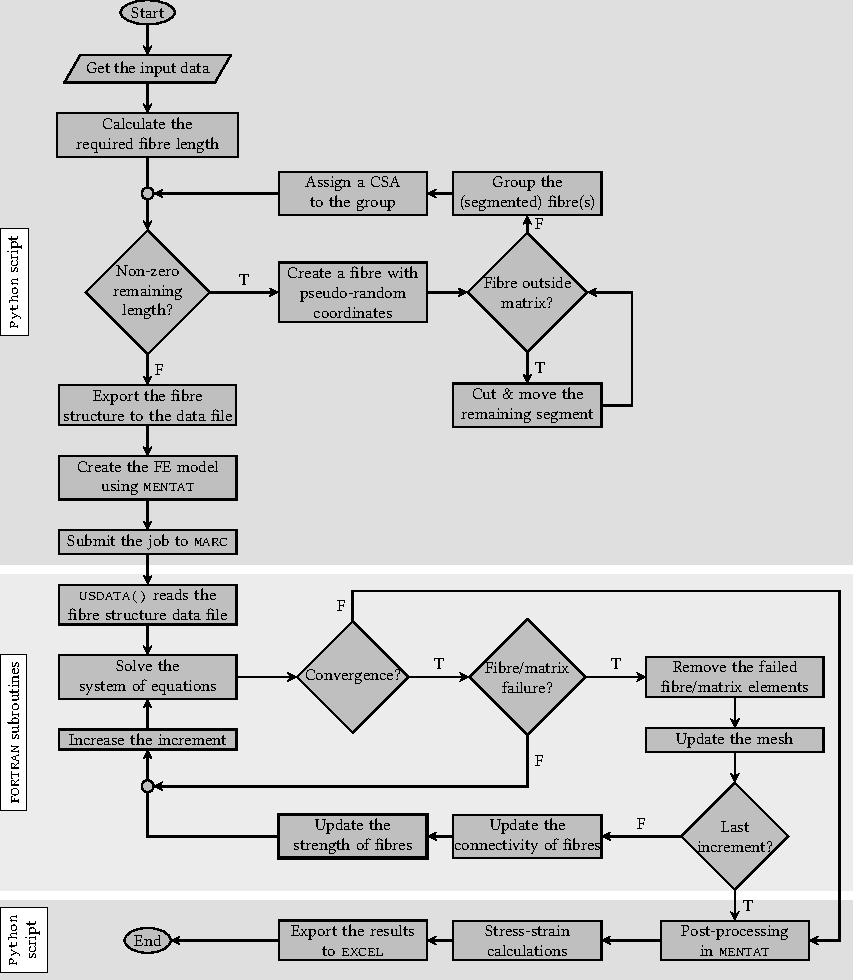
\includegraphics[width=\textwidth]{fig1_flowchart.pdf}
	\caption{Flowchart of the model creation, analysis, and post-process}\label{fig:m}
	\end{figure}
	A uniform mesh density was used throughout the model to facilitate the mesh sensitivity analyses. More specifically, the mesh density~\autocite{Javanbakht.2016b} is defined as
	\begin{equation}
		\gamma\equidef\frac{1}{\ell_\text{mesh}},
	\end{equation}
and controlled to obtain convergence while a single mesh length ($L_\text{mesh}$) is used for both fibre and matrix elements in the FE prototype. The number of elements used to represent each fibre depended on the fibre length, i.e., longer fibres consisted of more elements than shorter fibres in order to comply with a uniform mesh density. To this end, different length fibres were discretised into truss elements of the same size. A typical jute-epoxy FE model is shown in Fig.~\ref{fig:fe} in which the localised fibre/matrix failure region is enlarged.

	\begin{figure}[t!]%TODO add undamaged, damaged w/t and w/o the algorithm figures & write a qualitative (visual) description of the result
		\centering
		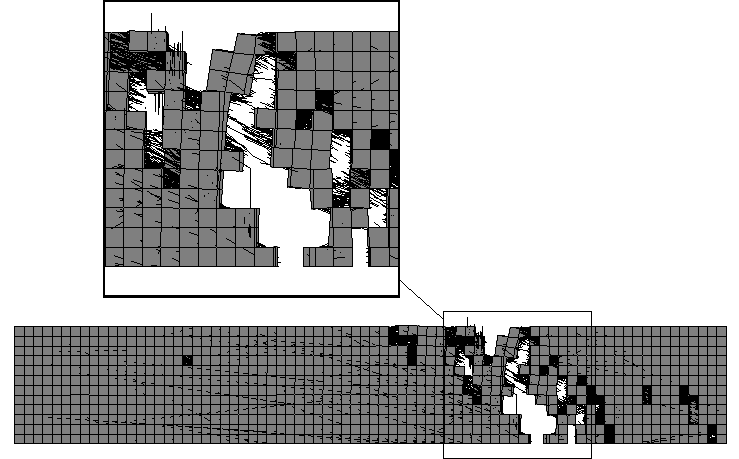
\includegraphics[width=\textwidth]{fig2_tensile_fe.pdf}
		\caption{Finite element model of a jute-epoxy composite sample upon failure (top view)}\label{fig:fe}
	\end{figure}

\subsection{Modelling Fibres}	
	The jute fibres and epoxy matrix were discretely modelled. Each fibre was represented using several simple truss elements (type 9) whilst 3D solid elements (type 7) were used to represent the matrix. The type 9 truss elements were two-node, single integration point elements with three translational degrees of freedom. The solid elements used in the matrix were eight-node isoparametric elements that utilised trilinear interpolation functions equipped with a full integration scheme. 
	
	The jute fibres were modelled as straight fibres with a constant CSA. Namely, technical fibres were modelled as a whole without considering individual elemental fibres, voids, resin impregnated volumes, or other internal structures. However the true shape of the cross-section was taken into consideration by means of the FACF. Since the elements are basically 1D, the Poisson's effect is also ignored.
	
	%TODO add a reference for the wall effect
	The distribution of the fibres satisfied material periodicity in order to avoid any wall effects.~\autocite{Miehe.2002} Although the distribution of fibres was quasi-unidirectional, they were allowed to penetrate through the walls of the matrix (sometimes called a soft boundary). Once a fibre penetrated the edge of the specimen, it was cut from the intersection point and the remaining segment is used to create a new fibre starting from the opposite edge. This arrangement was due to the fact that the tensile specimens were cut from a larger plate during manufacturing, and thus by following the explained procedure, the created samples better represent the parent material.
	
	% Do find references for softening
	Note that a quarter of the tensile specimen was considered instead of the whole specimen to reduce numerical load. Moreover, choosing an RVE was not considered since removing elements has a damage-like effect that results in softening of the response. An RVE---according to the ergodic hypothesis---must represent the whole structure over time. When very localised effects are present, e.g., softening in the form of degradation of elasticity, the RVE cannot present the whole structure that is showing a holistic behaviour. Namely, considering the whole structure is inevitable when various localised effects are present. In the current context, resin-rich areas and fibre clustering could make the unit cell approach not a good representation of the whole structure unless such imperfections are ignored. Finding an appropriate RVE by increasing the size of the realisations encounters convergence problems under softening behaviour and is still under investigation.~\autocite{Gitman.2007} This issue is closely related to the size effect issue that is mentioned in the introduction.
	
	
	The CSA for each fibre was selected from a log-normal distribution of the `true' fibre area~\autocite{Virk.2010b}. The `location' and `scale' parameters of 7.55 and 0.52 were used to characterise the true fibre CSA distribution, respectively. This log-normal distribution offers a realistic fit to the true cross-sectional area measurements of 106 jute fibres that were extracted from the same batch and were used to manufacture the jute-epoxy composite samples. Figure~\ref{fig:fibCSA} illustrates the possible discrepancy if the apparent CSA is used. These measurements were overlaid with the apparent and true log-normal CSA distribution for the jute fibres. 
	\begin{figure}[!t]
		\centering
%		\includegraphics[width=0.45\textwidth]{csa}
		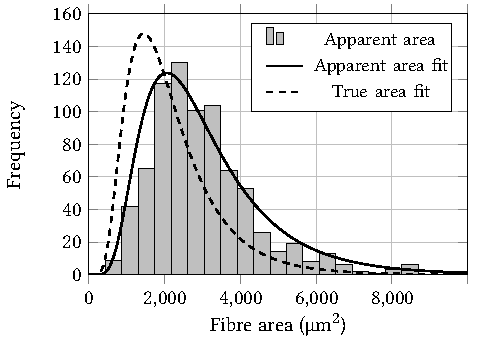
\includegraphics[scale=1]{fig3_area_dist}
		\caption{Fibre cross-sectional area distribution with $\text{FACF}=1.42$ (reproduced from~\autocite{Virk.2013})}\label{fig:fibCSA}
	\end{figure}
	
	The mechanical properties of the jute fibres, represented in the model, are influenced by fibre length~\autocite{Virk.2013, Virk.2009,Virk.2011}. Whilst the elastic modulus for the batch of jute fibres is relatively insensitive to fibre length, fracture strength and strain significantly reduce as fibre length increases~\autocite{Virk.2013b,Virk.2009}. Thus, to account for fibre length variations (and the interrelated mechanical properties), a log-normal distribution of fibre lengths was included with the location and scale parameters of 4.183 and 0.976, respectively. This log-normal distribution is representative of the fibre distribution resulting from 700 jute fibre measurements~\autocite{Virk.2009}. A comparison of the jute fibre length measurements and the log-normal fit (obtained using these location and scale parameters) is shown in Fig.~\ref{fig:len}.%TODO Proof-read until here

	\begin{figure}[!h]
		\centering
%		\includegraphics[width=0.50\textwidth]{len}
		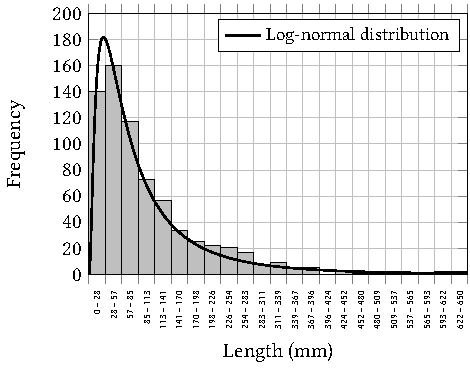
\includegraphics[scale=1]{fig4_len_dist}
		\caption{Fibre length distribution; reproduced from~\autocite{Virk.2009}}\label{fig:len}
	\end{figure}
		
	The elastic modulus of the jute fibres was taken (for each fibre) to be the mean of the 785 jute samples tested. This mean value (27.9\,GPa) is sensibly independent of fibre length~\autocite{Virk.2013}. In contrast, the failure strengths of the fibres were calculated based on fibre length and included in the FE models. The natural logarithmic interpolation model reported in~\autocite{Virk.2011} was used to calculate the fracture strengths for each fibre based on its length. The work of~\autocite{Virk.2011,Virk.2013} assumes a circular fibre cross-section. The elastic modulus and fracture strengths were therefore based on the apparent CSA. Thus, the FACF needed to be applied to both elastic modulus and failure strength of the fibres. A FACF of 1.42~\autocite{Virk.2010b} is included in the FE model for the elastic modulus and failure strength of the fibres as per Eqs.~\eqref{eq:enrom} and \eqref{eq:strengthcorrected}, respectively. Finally, the orientation of the fibres follows a Gaussian distribution, see Table~\ref{table:tests}. In this table, the mechanical properties and geometrical dimensions of five jute fibre reinforced composite samples (cases A--E) are summarised; they correspond to the experimental results in~\autocite{Virk.2013} (see the `Experimental Data' section for more details).

	% TABLE WITH 5 CASES [CASE B is omitted]
	\begin{table}[!th]
	\centering\small
	\caption{Measured mechanical properties of jute-epoxy composite (Plate values are the average values of the samples). Adapted from~\autocite{Virk.2013}.}\label{table:tests} 
	\begin{tabular}{lccccccc@{ }cc }% *{8}{>{\hfill}c}}
	\toprule
	\multicolumn{2}{l}{\multirow{2}{*}{\bfs{Property}}}&	
	\multicolumn{4}{c}{\bfs{Sample}}&
	&&\multicolumn{2}{c}{\bfs{Plate}}\\\cmidrule{9-10}\cmidrule{3-7}
	&&{\bfs{A}}	
	& {\bfs{B}}
	& {\bfs{C}}
	& {\bfs{D}}
	& {\bfs{E}}
	&&\bfs{Mean}	&\bfs{SD}\\
	\toprule
	\multicolumn{2}{l}{Width (mm)}		  				&25.14	&25.02	&25.06	&24.87	&25.03	&&25.05	&0.09\\
	\multicolumn{2}{l}{Thickness (mm)}					&3.15	&3.61	&3.67	&3.59	&3.67	&&3.52	&0.18\\
	\midrule
%	\multicolumn{2}{l}{Elastic modulus (GPa)}   		&8.98	&8.28	&7.79	&7.33	&8.70	&8.19	&0.55\\
%	\multicolumn{2}{l}{Tensile strength (MPa)}			&104.90	&99.60	&106.80	&94.80	&94.20	&100.06	&5.12\\
%	\multicolumn{2}{l}{Failure strain (\%)}				&1.26	&1.29	&1.40	&1.41	&1.15	&1.30	&0.10\\
	%\multicolumn{2}{l}{Poisson's ratio (longitudinal)}	&0.42	&0.42	&-		&0.44	&-		&0.42	&0.01\\\hline
	\multirow{2}{*}{Volume fraction (\%)}	&\ Mean		&17.50	&20.30	&20.90	&18.00	&18.50	&&18.88	&1.483\\
											& SD		&3.20	&3.80	&6.10	&3.10	&5.40	&&3.95	&n/a\\\midrule
	\multirow{2}{*}{Fibre angle ($^\circ$)}		&Mean	&5.72	&10.52	&7.90	&6.19	&6.59	&&7.36	&1.932\\
											&SD			&15.32	&18.44	&15.05	&16.09	&15.59	&&17.95	&n/a\\\midrule
	\multicolumn{2}{l}{$\eta_\text{o}$}					&0.86	&0.77	&0.85	&0.85	&0.85	&&0.81	&0.06\\
	\multicolumn{2}{l}{$\kappa$}			                        & 1.42&1.42&1.42&1.42&1.42&&1.42&0.00\\
	\multicolumn{2}{l}{$\eta_\text{d}$ or $\eta_\text{l}$}			& 1.00& 1.00& 1.00& 1.00& 1.00&&1.00&0.00\\
		\bottomrule
	\end{tabular}
	\end{table}

\subsection{Modelling the Matrix}
   	The fibres are modelled by means of two-node rod elements with linear shape functions. They are inserted into the matrix elements in a way that the degrees of freedom (DoFs) of the embedded elements take their values from those of the host (matrix) elements. The DoF values are interpolated based on the isoparametric location of the embedded node within the host. The mesh density of the matrix elements followed that of the fibres to facilitate the fibre embedding process ($\lambda=1$).
   	
   	Since the volume of the fibre elements is overlapped with that of the matrix elements, the volume of the matrix is artificially increased. Thus, a `virtual' thickness must be used instead of the real (original) thickness of the matrix:
   	\begin{equation}
   		t_\text{m,v}=(1-\zeta_\text{f})t_\text{m},
   	\end{equation}
   	where $t_\text{m}$ is the original matrix thickness and $t_\text{m,v}$ is the virtually decreased matrix thickness. Note that the volume fraction calculation is done with respect to the original thickness. A summary of the used properties is listed in Table~\ref{table:mech_p}. 
	
	\begin{table}[!b]
	\centering\small
	\caption{Summary of material properties}\label{table:mech_p}
	\begin{tabular}{p{0.1\textwidth}p{0.31\textwidth}p{0.5\textwidth}}
	\toprule
	\bfs{Material} 	& \bfs{Parameter} 	& \bfs{Value}\\
	\toprule
	Jute fibre		& Constitutive law				& Linear elastic, isotropic\\
					& Axial elastic modulus				& $27.9$ GPa~\autocite{Virk.2013} \\
					& Axial-radial Poisson's ratio				& $0.35$~\autocite{Virk.2016} \\
					& Failure criterion				& Maximum normal stress \\
					& Failure strength distribution	& Logarithmic interpolated Weibull distribution~\autocite{Virk.2011}\\
					& Characteristic strength&$\alpha_\text{log}=-111.656\ln(L_\text{fibre})+801.63$\, MPa\\ 
					& Shape parameter&$\beta_\text{log}=-0.152\ln(L_\text{fibre})+3.487$\\
					& Average axial fibre strength$^\dagger$ & $298.13\,\text{MPa}$\\
					& Fibre length distribution			& Log-normal ($\text{mean}=4.183$, $\text{SD}=0.976$)\\%(mean=65.6, STD=2.65)\\
					& CSA distribution				& Log-normal ($\text{mean}=7.55$, $\text{SD}=0.52$)\\%(mean=1900.74, STD=1.682)\\
					& Orientation distribution		& Gaussian ($\text{mean}=5$, $\text{SD}=10$) \\
					& Mean fibre orientation factor & $0.81\pm0.06$\\\midrule
	Epoxy			& Constitutive law				& Linear elastic, isotropic\\
					& Elastic modulus				& $2.65\,\text{GPa}$~\autocite{Virk.2013} \\
					& Poisson's ratio				& $0.35$~\autocite{Virk.2016} \\
					& Failure criterion				& Maximum normal stress\\
					& Failure strength				& $61\,\text{MPa}$~\autocite{Virk.2013}\\
					& Failure strain (\%)			& $4.1$~\autocite{Virk.2013}\\\midrule
	\multicolumn{3}{l}{$^\dagger$ The average axial strength corresponds to a fibre with average length in the distribution.}\\\bottomrule
	\end{tabular}
	\end{table}

%TODO back up using the max. shear stress critera by literature, READ the book that presented this
%TODO where exactly the FACF is applied in the model?

\subsection{Experimental Data}

	% description of experiments
	Experimental results in~\autocite{Virk.2013} were used as benchmark values. Five samples from a single jute fibre reinforced composite plate were cut, measured and prepared (five cases A--E). Micrographs (6--8 per sample) were taken to characterise the micro-structure of the samples, i.e., to estimate their volume fraction and the fibre orientation PDF by means of an image processing procedure. The statistical results were used to calculate the FODF and FACF for each sample. Since the diameter of the fibres were characterised accurately, a unit value was assigned to the fibre diameter distribution factor. In addition, the fibre length distribution factor was assumed to be equal to 1. The experimental results are summarised in Table~\ref{table:results}.



	% creating the validation models
	To account for the stochastic variations in fibre CSA, length and mechanical properties, as well as to accommodate the possible deviations in fibre orientation for the jute-epoxy composite samples, five pseudo-random realisations of the prototype were developed per case.  In each realisation, quasi-unidirectional fibres with variable length and CSAs were dispersed in a 3D matrix as per the distributions of Tables~\ref{table:tests} and~\ref{table:mech_p}. Moreover, each realisation was analysed twice: with updating the strength of the fibres and without strength updating. The simulations were carried out for jute fibre-reinforced composite samples with low fibre volume fractions (in the range 17.5--20.9 vol\%). A total of 50 probabilistic FE models were therefore considered. The stress-strain curve for one of the realisations of Case D is depicted in Fig.~\ref{fig:stressstrain}.

	\begin{figure}[!t]
		\centering
		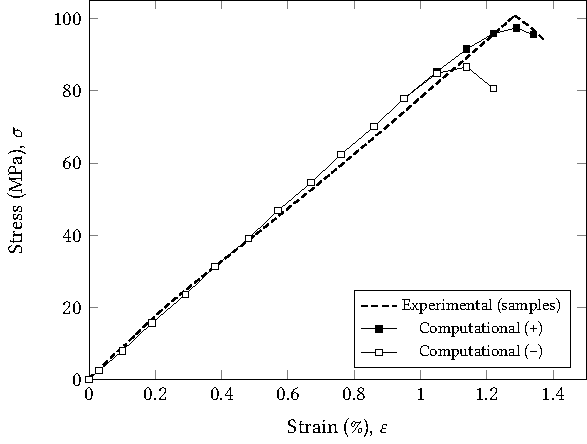
\includegraphics[scale=1]{fig5_fea_vs_test.pdf}
		\caption{Stress-strain response for a single realisation of Case D with $V_\text{f}=18\%$ (the $+$ and $-$ symbols denote the `with strength updating' and `without strength updating' algorithms, respectively)}\label{fig:stressstrain}
	\end{figure}%
In summary, in order to have a model that statistically represent the real specimens, the computer-generated prototype provides the following capabilities:
\begin{itemize}
\item discrete modelling of embedded fibres;
\item generating arbitrary volume fractions;
\item controlling various statistical features, e.g., the length, CSA, strength, and the orientation distribution of the fibres;
\item generating and updating length-dependent strength according to the Weibull distribution; 
\item applying the relevant correction factors to the material properties, e.g., FACF to natural fibres; 
\item applying the volumetric correction factor (by means of a virtual thickness) to compensate for the volume of the embedded fibres in the matrix; and
\item applying element elimination technique to both matrix and fibre elements based on the maximum stress failure criterion (implementing other criteria is also possible).
\end{itemize}
	

\section{Results and Discussion}
	A total of 25 realisations were analysed; first with updating the strength of fibres, and then without this consideration. The simulations were carried out according to the statistical results obtained from experiments, i.e., the same volume fractions, fibre angle orientation distributions, fibre CSA distributions, and fibre length distributions were used. Elastic modulus, tensile strength, and failure strain of the simulations were calculated and illustrated in Fig.~\ref{fig:main_results}. The values and their corresponding percentage relative differences are available in Table~\ref{table:results}. Obviously, the obtained values are bound to the limitations of pseudo-random model generation. Nevertheless, some useful derivations are obtained by analysing them.

	
\begin{figure}[!t]{}
  	\centering
  	\subfloat[][Elastic moduli\label{fig:E}]{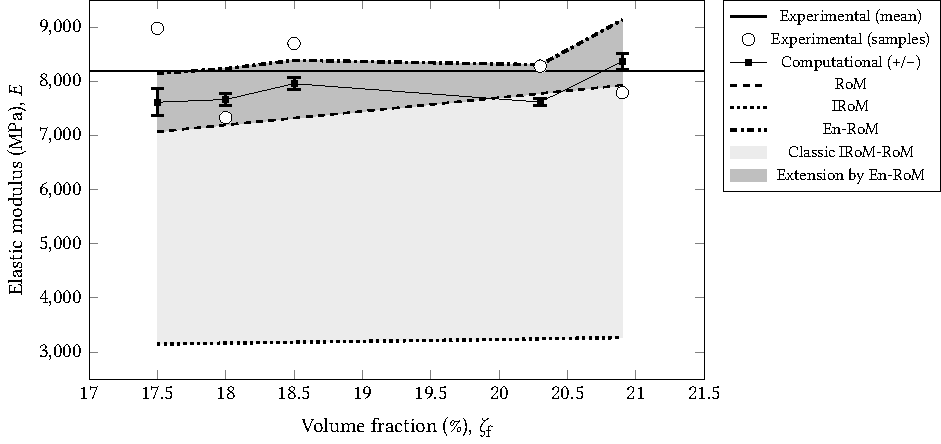
\includegraphics[height=0.28\textheight]{fig6a_E}}\\
  	\subfloat[][Tensile strength\label{fig:stress}]{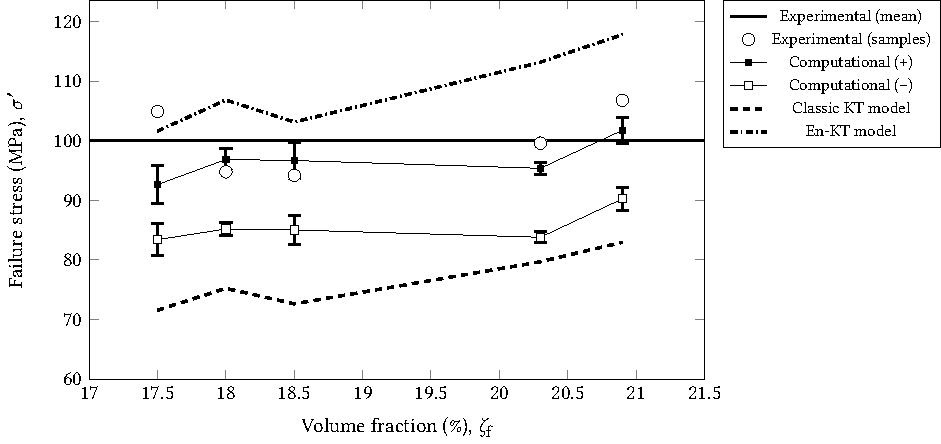
\includegraphics[height=0.28\textheight]{fig6b_strength}}\\
 	\subfloat[][Failure strain\label{fig:strain}]{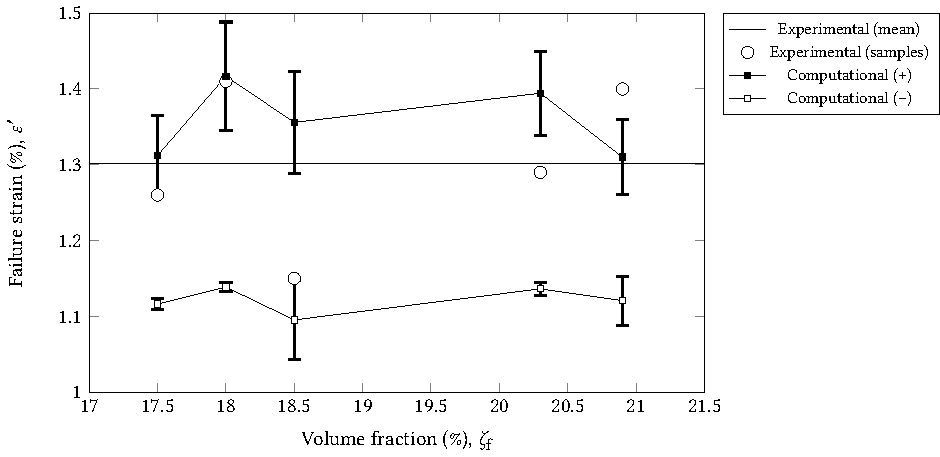
\includegraphics[height=0.28\textheight]{fig6c_failure_strain}}\\
	\caption{Results of experimental, computational, and analytical models (the $+$ and $-$ symbols denote the `with strength updating' and `without strength updating' algorithms, respectively).}
	\label{fig:main_results}
\end{figure}%
\afterpage{\clearpage}


	\paragraph{Elastic modulus} The experimental values for the elastic moduli were outside the range predicted by the classic IRoM and RoM, see the lightly shaded region in Fig.~\ref{fig:E}. The estimated upper value by RoM is extended by means of the En-RoM according to Eq.~\eqref{eq:enrom}; the extended region is shaded slightly darker in the figure. Moreover the averaged value of the specimens---the black horizontal line that corresponds to the plate value---resides mostly in the area that is extended by the En-RoM. The elastic moduli obtained from the numerical analyses were insensitive to updating the strength of the fibres as both computational values overlap. Similar to the experimental results, the computational values are mostly in the extended region. If the plate value is taken as the representative of the material, the computational approach seems to slightly underestimate the stiffness (average relative difference of $-$4.53\%) whereas the classic analytical estimates barely meet the experimental values (average relative difference of $-$9.72\%). On the other hand, the En-RoM estimates the elastic modulus very closely with an average relative difference of 0.26\%. 

	
\begin{table}[!t]
\centering\scriptsize
\def\GPa{{\scriptsize (GPa)}}
\caption{Experimental, numerical and analytical results for elastic modulus ($E$, in GPa), tensile strength ($\sigma^\prime$, in MPa) , and failure strain~($\varepsilon^\prime$, in percentage).}\label{table:results}
\begin{tabular}{p{0.07\textwidth}@{}*{5}{@{}S@{}>{\scriptsize\,}l@{}}@{}S@{}>{\scriptsize\,}l@{}@{}S@{}}
	\toprule
	\multirow{2}{*}{\bfs{Property}}   &                                                            \multicolumn{10}{c}{\bfs{Case}}                                                            &                 \multicolumn{3}{c}{\bfs{Plate}}                 \\
	\cmidrule(l{0.3cm}r{0cm}){12-14}\cmidrule(l{0.3cm}r{0cm}){2-11} & \multicolumn{2}{c}{{\bfs{A}}} & \multicolumn{2}{c}{{\bfs{B}}} & \multicolumn{2}{c}{{\bfs{C}}} & \multicolumn{2}{c}{{\bfs{D}}} & \multicolumn{2}{c}{{\bfs{E}}} & \multicolumn{2}{c}{{\bfs{Mean}}} & {\bfs{SD (\%)}} \\ \toprule
	$E_\text{Exp}$                  & 8.98    &                 & 8.28    &               & 7.79    &              & 7.33    &              & 8.70    &              & 8.19    &              & 8.16             \\
	$E_{+/-}$                       & 7.615   & [$-15.20$]      & 7.616   & [$-8.01$]     & 8.367   &   [$+7.40$]  & 7.665   & [$+4.57$]    & 7.957   & [$-8.54$]    & 7.844   & [$-4.53$]    & 4.14      \\
	$E_\text{RoM}$                  & 7.068   & [$-21.28$]      & 7.776   & [$-6.09$]     & 7.927   &  [$+1.76$]   & 7.195   & [$-1.84$]    & 7.321   &  [$-15.85$]  & 7.417   &  [$-9.72$]   & 5.05      \\
	$E_\text{En-RoM}$               & 8.149   & [$-10.20$]      & 8.305   & [$+0.30$]     & 9.134   & [$+14.72$]   & 8.235   & [$+10.98$]   & 8.390   & [$-3.70$]    & 8.208   & [$+0.26$]    & 4.83   \\ 
	$E_\text{IRoM}$                 & 3.148   &                 & 3.246   &               & 3.268   &              & 3.165   &              & 3.182   &              & 3.196   &              & 1.63             \\\midrule
	$\sigma^\prime_\text{Exp}$      & 104.90  &                 & 99.60   &               & 106.80  &              & 94.80   &              & 94.20   &              & 100.06  &              & 8.26              \\
	$\sigma^\prime_{+}$             & 92.652  & [$-11.68$]      & 95.381  & [$-4.24$]     & 101.768 &  [$-4.71$]   & 96.870  & [$+2.18$]    & 96.686  &  [$+2.64$]   & 96.671  &  [$-3.39$]   & 3.42         \\
	$\sigma^\prime_{-}$             & 83.401  & [$-20.49$]      & 83.810  & [$-15.85$]    & 90.258  &  [$-15.49$]  & 85.214  & [$-10.11$]   & 85.039  &  [$-9.73$]   & 85.545  &   [$-14.51$] & 3.21            \\
	$\sigma^\prime_{\text{KT}}$     & 71.572  & [$-31.77$]      & 79.707  & [$-19.97$]    & 82.976  &  [$-22.31$]  & 75.240  & [$-20.63$]   & 72.645  &  [$-22.88$]  & 75.997  &   [$-24.05$] & 6.34            \\
	$\sigma^\prime_{\text{En-KT}}$  & 101.632 & [$-3.12$]       & 113.184 & [$+13.64$]    & 117.825 & [$+10.32$]   & 106.841 & [$+12.70$]   & 103.156 &  [$+9.51$]   & 107.916 &  [$+7.85$]   & 6.34            \\ \midrule
	$\varepsilon^\prime_\text{Exp}$ & 1.2600  &                 & 1.2900  &               & 1.4000  &              & 1.4100  &              & 1.1500  &              & 1.3020  &              & 0.85            \\
	$\varepsilon^\prime_+$          & 1.3120  & [$+4.13$]       & 1.3944  & [$+8.10$]     & 1.3101  & [$-6.42$]    & 1.3558  & [$+0.48$]    & 1.3558  & [$+17.90$]   & 1.3578  & [$+4.29$]    & 0.37    \\
	$\varepsilon^\prime_-$          & 1.1162  & [$-11.42$]      & 1.1363  &  [$-11.91$]   & 1.1207  &  [$-19.95$]  & 1.0953  & [$-19.24$]   & 1.0953  & [$-4.76$]    & 1.1214  & [$-13.87$]   & 0.02     \\ \midrule
	\multicolumn{14}{l}{\scriptsize Note 1.\quad The $+$ and $-$ subscripts denote the `with strength updating' and `without strength updating' algorithms, respectively.}                                                                                                   \\
	\multicolumn{14}{l}{\scriptsize Note 2.\quad  Values in brackets denote the percentage relative difference with respect to the corresponding experimental value.}                                                                                                                                                                                              \\ 
	\multicolumn{14}{l}{\scriptsize Note 3.\quad  The `SD (\%)' is the SD normalised with respect to the mean value---it is also called percent deviation from mean Value.}                                                                                                                                                                                              \\ \bottomrule
\end{tabular}
\end{table}

	\paragraph{Tensile strength} The experimental values for ultimate strength lie between the estimated analytical values: the classic Kelly-Tyson underestimates the failure strength of the tensile specimens whereas its extended version provides much better estimations (average relative difference of 7.85\%). This improvement is mainly due to incorporating the FACF into the classical version, see Eq.~\eqref{eq:en-KT}. The numerical models with strength updating provide the best approximation with an average relative difference of $-$3.39\%. This result is a substantial improvement to the $-$14.51\% relative difference of the numerical models that discard strength updating. Considering the average experimental value (the black horizontal line in Fig.~\ref{fig:stress}), the computational models still underestimate the overall behaviour whereas the En-KT model overestimates the strength. This overestimation was expected since the microstructural defects present in the experimental material is not considered in En-KT. It is worth mentioning that most of the numerical results with strength updating exhibit only small deviations from the mean value.
	

	\paragraph{Failure strain} The experimental values show an average of 1.30\% for the failure strain. The numerical models without strength updating underestimate the experimental value of the failure strain (average relative difference $-$13.87\%) whereas for the case of the strength updating models, a slight overestimation of about 4.29\% average relative difference is obtained. The rather brittle response of the models without fibre strength updating is due to the sudden removal of several elements in a single increment. By removing the strength updating, all elements of a fibre inherit the same strength irrespective of their updated length. Thus, most of the elements of a failing fibre are removed, concurrently. On the other hand, strengthening of the subdivided fibres result in a more ductile response and allows the stress field to grow more smoothly within the composite and engage more fibres before failure. This also justifies the higher strength values of the updating models.
	
	\paragraph{Consistency of results} In the last column of Table~\ref{table:results}, the percent deviation from the mean value is presented for the results. It is evident that the strength updating approach provides pretty consistent results in terms of estimating elastic modulus (4.14\%), failure strength (3.42\%), and failure strain (0.37\%). These values are greater than their corresponding experimental values, i.e., 8.16\%, 8.26\%, and 0.85\%, respectively. These results emphasises that the numerical algorithm could produce consistent results according to the input statistical distributions. The same statement is valid for the algorithm without strength updating, albeit those results show a higher relative difference with respect to the experimental findings. Finally, among the estimated values, the failure strain has received the most consistent results (0.37\% and 0.02\%). Obviously, increasing the number of realisations renders the average of the results a better representation of the physical specimens.
	


\section{Conclusion}
	The current work aimed to illustrate the importance of incorporating FACF in both analytical and numerical models. Moreover, a methodology for creating embedded natural fibres within a composite and mimicking the damage evolution is described. The proposed algorithm is novel for implementing the following innovations:
	\begin{itemize}
	\item computational incorporation of length-dependent strength response of fibres (in the spirit of fracture mechanics), by updating the strength of fibre elements upon failure during the FE analyses,
	\item implicit modelling of damage by element elimination techniques without requiring specific characterisation of damage parameters,
	\item using a virtual thickness for the specimens to adjust the volumetric discrepancy of the matrix due to embedding discrete fibres, and
	\item numerical implementation of fibre cross-section non-uniformity using a correction factor to fine-tune the apparent fibre CSA.
	\end{itemize}
	Cross-sectional area measurement of non-circular natural fibres---while assuming a perfect circular cross-section---overestimates the true values. Thus, calculation of strength and stiffness of technical fibres would be an underestimation of the real values. This subtle point should be reflected in both analytical and numerical models. To this end, the classic Kelly-Tyson model and RoM were extended to their enhanced versions and an algorithm for discrete modelling of natural fibres was provided. All the suggested amendments improved the original results that ignored the FACF. 
	
	Considering that linear material models were used, the non-linear response of the NFC is implicitly allowed. Namely, the discrete modelling of fibres and the technique of removing the failed elements during the analysis were the means for including the gradual material deterioration during the loading. However, updating the strength of the fibres according to their length after failure showed a substantial improvement in estimating the tensile strength and failure stress. When the strength updating is dropped, the response of embedded fibres become more brittle and the strength of the composite is underestimated since a more localised failure is induced. On the other hand, the elastic modulus remained insensitive to fibre strength updating.
	
	The introduced method can be used in multi-scale modelling to set up a simple representative volume element with embedded fibres in the meso-scale. In addition, the computational models can be further improved by considering non-local continua formulation for the composite to smooth the damage propagation and alleviate the artificial stress concentration due to sudden fibre removal.


